\documentclass{article}

\usepackage{amsmath, amsthm, amssymb, amsfonts}
\usepackage{thmtools}
\usepackage{graphicx}
\usepackage{setspace}
\usepackage{geometry}
\usepackage{float}
\usepackage{hyperref}
\usepackage[utf8]{inputenc}
\usepackage[english]{babel}
\usepackage{framed}
\usepackage[dvipsnames]{xcolor}
\usepackage{tcolorbox}

\colorlet{LightGray}{White!90!Periwinkle}
\colorlet{LightOrange}{Orange!15}
\colorlet{LightGreen}{Green!15}

\newcommand{\HRule}[1]{\rule{\linewidth}{#1}}

\newtheorem{theorem}{Theorem}[section]
\newtheorem{lemma}[theorem]{Lemma}

\theoremstyle{definition}
\newtheorem{definition}{Definition}[section]

\setstretch{1.2}
\geometry{
    textheight=9in,
    textwidth=5.5in,
    top=1in,
    headheight=12pt,
    headsep=25pt,
    footskip=30pt
}

% ------------------------------------------------------------------------------

\begin{document}

% ------------------------------------------------------------------------------
% Cover Page and ToC
% ------------------------------------------------------------------------------

\title{ \normalsize \textsc{}
		\\ [2.0cm]
		\HRule{1.5pt} \\
		\LARGE \textbf{\uppercase{Ergodic Theory}
		\HRule{2.0pt} \\ [0.6cm] \LARGE{MATH 470 Report} \vspace*{10\baselineskip}}
		}
\date{}
\author{\textbf{Samy Lahlou Kamal} \\ 
		  Montreal, Canada \\
		Summer 2024}

\maketitle
\newpage

\tableofcontents
\newpage

% ------------------------------------------------------------------------------

\section{Introduction}

In this report, I will summarize the topics I have covered with Professor Anush Tserunyan and Kaining Jia during the summer 2024. The main topic was Ergodic Theory, but we focused on the Birkhoff Ergodic Theorem, some variations and generalizations (using group actions) as well as new proof methods including the tilings and boundary actions.\\
I will not write everything I learned during the summer in this report because I also had to learn about Measure Theory and did a lot of exercises on the Riemann Integral and Functional Analysis. \\

\section{Some Useful Definitions}

\subsection{Measure Theory}
It would be hard to read this report without some background in measure theory. However, I will still recall some useful definitions since the main structures we will deal with here are probability measure spaces.

\begin{definition}[Measure space and Probability Measure Space]
    Let $X$ be a set, $\beta \subset 2^X$ be a $\sigma$-algebra on $X$ and $\mu : \beta \to X$ be a function, then the triplet $(X,\beta, \mu$) is a \textit{measure space} if :
    \begin{itemize}
        \item $\mu (\emptyset) = 0$
        \item $\mu \left( \bigcup E_n \right) = \sum_{n=0}^{\infty}\mu(E_n)$ for any pairwise disjoint collection $\{E_n\}_{n\in\mathbb{N}}\subset\beta$
    \end{itemize}
    Moreover, we say that $(X,\beta, \mu)$ is a \textit{probability measure space} if $$\mu (X) = 1$$ We refer to the elements of $\beta$ as \textit{measurable} sets.\\
\end{definition}

Sometimes, we can simply refer to a probability measure space as a \textit{probability space}. Moreover, if the $\sigma$-algebra is clear from the context, we can simply refer to $(X,\beta,\mu)$ as $(X,\mu)$.\\
Some standard probability measure space are $([0,1), \lambda)$, where $\lambda$ is the Lebesgue Measure, or $(2^{\mathbb{N}}, \{\frac13,\frac23\}^{\mathbb{N}})$.

Another key tool that will be used very often here are the measurable functions and transformations.

\begin{definition}
    Let $(X,\beta_1,\mu_1)$ and $(Y,\beta_2,\mu_2)$ be measure spaces and $f:X\to Y$ be a function. Then $f$ is $(\beta_1,\beta_2)$-\textit{measurable} if $$f^{-1}B\in\beta_1$$ for all $B\in\beta_2$. If the $\sigma$-algebras are clear from the context, then we simply say that $f$ is \textit{measurable}.\\
\end{definition}

Again, as an example, the baker's map $b:[0,1)\to [0,1)$ is a measurable transformation if the measure is the Lebesgue measure $\lambda$. Another example would be the shift $\sigma :2^\mathbb{N} \to 2^\mathbb{N}$ defined by $(x_n)\mapsto (x_{n+1})$ where the measure is $\{ \frac12,\frac12 \}^{\mathbb{N}}$.

\subsection{Basics of Ergodic Theory}

In this subsection, fix a probability space $(X, \mu)$. Here, I will define all notions that will let us define and understand the notion of ergodicity, which is the main notion of the report. \\
Ergodicity can be defined for any measurable transformation $T$ but we will only focus here on probability measure preserving transformations since the main theorems only apply to these transformations.

\begin{definition}[Probability Measure Preserving]
A measurable transformation $T:X\to X$ is \textit{probability measure preserving} if $$\mu(T^{-1}B)=\mu(B)$$ for any measurable set $B$. It will be easier to refer to this property as \textit{pmp}.\\
\end{definition}

This definition is not hard to understand and is self-contained in its name. A pmp transformation preserves the measure of a set. A very basic example would be a translation or rotation with the Lebesgue measure on $\mathbb{R}^2$. The next definition is similar.

\begin{definition}[T-invariance for sets]
    For a measurable transformation $T:X\to X$, a set $B\subset X$ is $T$-\textit{invariant} if $$T^{-1}B=B$$
\end{definition}

A set is $T$-invariant when its elements simply get \textit{shuffled} by $T$. An easy example would by any rotation applied to any circle centered at zero. We can define the notion of $T$-invariance for functions as well.

\begin{definition}[T-invariance for functions]
    For a measurable transformation $T:X\to X$, a function $f:X\to \mathbb{R}$ is $T$-\textit{invariant} if $$f=f\circ T$$ Equivalently, it is not hard to prove that $f$ is $T$-invariant if $f^{-1}(A)$ is a $T$-invariant set for all $A \subset \mathbb{R}$.
\end{definition}

With all of these definitions in hand, we are now able to define the notion of ergodicity. 

\begin{definition}[Ergodicity]
    Let $T:X\to X$ be a measurable transformation, then $T$ is \textit{ergodic} if every $T$-invariant measurable set is null or conull, i.e, $\mu(B) \in \{0,1\}$ for all $T$-invariant measurable set $B$
\end{definition}

A transformation is ergodic if we cannot decompose the space $X$ into positive measure invariant subsets. As for prime numbers or a lot of other notions in mathematics, ergodicity has something to do with some elements being decomposable or not.\\
Since invariance is important when defining ergodicity and invariance is defined for both sets and functions, we can deduce an ergodicity criterion using invariance of functions.

\begin{theorem}[Ergodicity Criterion]\label{Criterion}
    A measurable transformation  $T:X\to X$ is ergodic iff every $T$-invariant measurable function $f:X\to \mathbb{R}$ is constant a.e on $X$.
\end{theorem}

\begin{proof}
    ($\Rightarrow$) Suppose that $T$ is ergodic and let $f\in L^1(X,\mu)$ be $T$-invariant, let's show that $f$ is constant a.e on $X$.
    Consider the sets $A,B\subset\mathbb{R}$ defined as
    \begin{align*}
        A &:= \{a\in\mathbb{R}:\mu(f^{-1}(a,\infty))=0\} \\
        B &:= \{b\in\mathbb{R}:\mu(f^{-1}(-\infty,b])=0\}
    \end{align*}
    First, let's show that $A$ and $B$ are disjoint. By contradiction, suppose that there exists an $x\in\mathbb{R}$ such that $x\in A\cap B$, then 
    \begin{align*}
        &\mu(f^{-1}(x,\infty))=0 \\
        &\mu(f^{-1}(-\infty,x])=0
    \end{align*}
    So we get
    \begin{align*}
        \mu(X) &= \mu(f^{-1}(\mathbb{R})) \\
          &= \mu(f^{-1}((-\infty,x]\cup (x,\infty))) \\
          &= \mu(f^{-1}(-\infty,x])\cup f^{-1}(x,\infty)) \\
          &= \mu(f^{-1}(-\infty,x])+ \mu(f^{-1}(x,\infty)) \\
          &= 0 + 0 \\
          &= 0
    \end{align*}
    A contradiction, so $A\cap B = \emptyset$.
    Let's now prove that $\mathbb{R} = A\cup B$. Let $x\in \mathbb{R}\setminus A$, then $\mu(f^{-1}(-\infty, x])\neq 0$. By ergodicity of $T$ and by the $T$-invariance of $f$, $f^{-1}(-\infty, x]$ is $T$-invariant and measurable, so we must have $\mu(f^{-1}(-\infty, x])=1$. Thus,
    \begin{align*}
        & \mu(X) = \mu(f^{-1}(-\infty,x])+ \mu(f^{-1}(x,\infty)) \\
        \implies   & 1 = 1 + \mu(f^{-1}(x,\infty))\\
        \implies  & \mu(f^{-1}(x,\infty)) = 0\\
        \implies & x\in B
    \end{align*}
    Hence, $\mathbb{R} = A\cup B$. Let's now prove that both $A$ and $B$ are nonempty. Suppose that $B=\emptyset$, then $A=\mathbb{R}$. In this case $n\in A$ for all $n\in \mathbb{N}$:
    
    \begin{align*}
        \mu(X) &= \mu(f^{-1}(\mathbb{R})) \\
          &= \mu \left( f^{-1} \left( \bigcup_{n=0}^{\infty}(-\infty,n] \right) \right) \\
          &= \mu \left( \bigcup_{n=0}^{\infty} \left( f^{-1} (-\infty,n] \right) \right) \\
          & \leq \sum_{n=0}^{\infty} \mu \left(f^{-1} (-\infty,n] \right) \\
          &= \sum_{n=0}^{\infty} 0 \\
          &= 0
    \end{align*}

    Thus, $B$ is nonempty. Similarly, $A$ is nonempty as well. Finally, let's show that if $a_0\in A$ and $a\leq a_0$, then $a\in A$:
    \begin{align*}
        & a \leq a_0 \\
        \implies & (-\infty, a] \subset (-\infty, a_0] \\
        \implies & f^{-1}(-\infty, a] \subset f^{-1}(-\infty, a_0] \\
        \implies & \mu(f^{-1}(-\infty, a]) \leq \mu(f^{-1}(-\infty, a_0]) = 0 \\
        \implies & \mu(f^{-1}(-\infty, a]) = 0\\
        \implies & a \in A
    \end{align*}

    Similarly, if $b_0\in B$ and $b_0\leq b$, then $b\in B$. Using these properties of $A$ and $B$, it follows by Completeness of $\mathbb{R}$ that there exists a $c\in \mathbb{R}$ such that $(-\infty, c)\subset A$ and $(c, \infty) \subset B$ ($c = \sup(A) = \inf(B)$). Now, it remains to show that $f(x)=c$ for a.e $x\in X$, to do this, we will show equivalently that $\mu(f^{-1}(\mathbb{R}\setminus \{c\}))=0$:

    \begin{align*}
        \mu(f^{-1}(\mathbb{R}\setminus \{c\})) &=  \mu(f^{-1}(-\infty,c)\cup f^{-1}(c, \infty)) \\
          &= \mu(f^{-1}(-\infty,c)) +  \mu(f^{-1}(c, \infty)) \\
          &= \mu \left(f^{-1} \bigcup_{n=1}^{\infty}(-\infty, c-\frac1n]\right) + \mu \left(f^{-1} \bigcup_{n=1}^{\infty}(c+\frac1n, \infty)\right)\\
          &\leq \sum_{n=1}^{\infty}\mu(f^{-1}(-\infty, c-\frac1n]) + \sum_{n=1}^{\infty}\mu(f^{-1}(c+\frac1n, \infty)) \\
          &= \sum_{n=1}^{\infty}0 + \sum_{n=1}^{\infty}0 \\
          &= 0
    \end{align*}

    This concludes the first part of the proof.\\
    ($\Leftarrow$) Suppose now that every $T$-invariant measurable function $f:X\to\mathbb{R}$ is constant a.e on $X$. Let's show that $T$ is ergodic. Let $B\subset X$ be a $T$-invariant measurable set and consider the function $\chi_B:X\to\mathbb{R}$. Since $B$ is measurable, then $\chi_B$ is measurable as well. Let $x\in X$, since $T^{-1}B=B$, we must have $\chi_B(x)=\chi_B(T(x))$, so $\chi_B$ is $T$-invariant. By our assumption on $T$-invariant measurable functions, $\chi_B$ is a.e constant. If $\chi_B(x)=1$ for a.e $x\in X$, then $B$ is conull. If $\chi_B(x)=0$ for a.e $x\in X$, then $B$ is null. Therefore, $T$ is ergodic.
\end{proof}

This criterion will be very useful when proving the Birkhoff Ergodic Theorem.


\section{Ergodic Theorems}
\subsection{Birkhoff Ergodic Theorem}

Let $(X,\mu)$ be a probability space with a pmp transformation $T:X\rightarrow X$.\\
In this subsection, we will focus on the Birkhoff Ergodic Theorem and prove it. To prove this theorem, we will first define a few functions and prove two important lemmas : the local-global bridge and the $T$-invariance of $\overline{f}$ and $\underline{f}$ (which will be defined later).

\begin{theorem}[Birkhoff Ergodic Theorem]\label{Birkhoff}
    T is ergodic iff for each $f \in L^1(X,\mu)$ and a.e $x\in X$,
    $$\lim_{n\to\infty}\frac{1}{n+1}\sum_{i=0}^n(f\circ T^i)(x)=\int_Xfd\mu$$
\end{theorem}

What this theorem says is that ergodicity implies that for almost every point $x$ in the space $X$, the \textit{forward orbit of $x$}, $\{x, Tx, T^2x, ...\} = \{T^nx : n\in\mathbb{N}\}$ is enough to sample every part of the space. Moreover, $T$ being pmp makes this sampling of $X$ uniform enough to give us arbitrarily precise approximations of $\int_Xfd\mu$ for any $f\in L^1(X,\mu)$.

\begin{definition}
    For a function $f\in L^1(X,\mu)$ and $n\in \mathbb{N}$, define $A_nf:X\to \mathbb{R}$ by
    $$A_nf(x) = \frac{1}{n+1}\sum_{i=0}^n(f\circ T^i)(x)$$
    for $x\in X$. For a fixed $x\in X$, $A_nf(x)$ is the average of $f$ over $x, Tx, T^2x, ...,T^nx$.
\end{definition}

\begin{lemma}[Local-global bridge]
    For all $f\in L^1(X,\mu)$ and any natural number $n\geq 1$,
    $$\int_Xfd\mu = \int_XA_nfd\mu$$
\end{lemma}

\begin{proof}
    Let $f\in L^1(X,\mu)$ and $n\geq 1$. Let's first show that $$\int_X(f\circ T)d\mu = \int_Xfd\mu$$. Since $T$ is pmp, for any measurable set $B\in \beta$:
    $$(T_*\mu)(B)=\mu(T^{-1}B)=\mu(B)$$
    so $T_*\mu=\mu$. Thus, using the change-of-variable formula :
    $$ \int_X(f\circ T)d\mu = \int_Xfd(T_*\mu) = \int_Xfd\mu$$
    Hence, by induction on $i\in \mathbb{N}$:
    $$ \int_X(f\circ T^i)d\mu = \int_Xfd\mu$$
    Therefore,
    \begin{align*}
        \int_XA_nfd\mu &= \int_X \frac{1}{n+1}\sum_{i=0}^n(f\circ T^i) d\mu\\
        &= \frac{1}{n+1}\sum_{i=0}^n \int_X(f\circ T^i) d\mu\\
        &= \frac{1}{n+1}\sum_{i=0}^n \int_Xfd\mu\\
        &= \frac{n+1}{n+1}\int_Xfd\mu\\
        &= \int_Xfd\mu
    \end{align*}
    
\end{proof}

The statement of the Ergodic Theorem deals with the function $x\mapsto \lim_{n\to\infty}A_nf(x)$, hence, it is clear to see the role that the next definition will play in the proof of the theorem.

\begin{definition}
    For a function $f\in L^1(X,\mu)$, define the functions $\overline{f}$ and $\underline{f}$ by
    $$\overline{f}(x)=\limsup_nA_nf(x)$$
    and
    $$\underline{f}(x)=\liminf_nA_nf(x)$$
    for $x\in X$.
\end{definition}

\begin{lemma}[Invariance of $\overline{f}$ and $\underline{f}$]\label{Invariance}
    For all $f\in L^1(X,\mu)$, the functions $\overline{f}$ and $\underline{f}$ are $T$-invariant.
\end{lemma}

\begin{proof}
    Let $x\in X$ :
    \begin{align*}
        (\overline{f}\circ T)(x) &= \limsup_nA_nf(Tx) \\
        &= \limsup_n\frac{1}{n+1}\sum_{i=0}^n(f\circ T^{i+1})(x) \\
        &= \limsup_n\frac{1}{n+1} \left( \sum_{i=0}^{n+1}(f\circ T^i)(x) -f(x)\right) \\
        &= \limsup_n \left( \frac{n+2}{n+1}A_{n+1}f(x) -\frac{1}{n+1}f(x)\right) \\
        &= \limsup_nA_{n+1}f(x) \\
        &= \limsup_nA_nf(x) \\
        &= \overline{f}(x)
    \end{align*}
    So $\overline{f}$ is $T$-invariant. Similarly, $\underline{f}$ is $T$-invariant as well.
\end{proof}

Let's now prove the Ergodic Theorem.

\begin{proof}
    ($\Rightarrow$) Suppose that $T$ is ergodic and let's show using a tiling argument that $$\lim_{n\to\infty}\frac{1}{n+1}\sum_{i=0}^n(f\circ T^i)(x)=\int_Xfd\mu$$
    for all $f\in L^1(X,\mu)$ and a.e $x\in X$. Let $f\in L^1(X,\mu)$, then u   sing Lemma \ref{Invariance} and the Ergodicity Criterion \ref{Criterion}, both $\overline{f}$ and $\underline{f}$ are constant a.e on $X$. WLOG, we will suppose that $$\int_Xfd\mu = 0$$
    By way of contradiction, suppose that $\overline{f} > 0$ (a.e), then there must be a $\Delta > 0$ s.t $$\overline{f} > \Delta > 0$$. Hence, we can define the function $x\mapsto n_x$ which maps $x$ to the least positive integer $n_x$ satisfying $A_{n_x}f(x)>\Delta$. We will assume here that $x\mapsto n_x$ is bounded by some $l>0$ and that $f$ is bounded as well. Let $\epsilon >0$ and define $N\in \mathbb{N}$ such that $l/(N+1) < \epsilon$, then for all $x\in X$,
    \begin{align*}
        A_Nf(x) &= \frac{1}{N+1}\left( f(x) + f(Tx) + ... + f(T^Nx) \right) \\
        & > \frac{1}{N+1}\left( \Delta n_x + \Delta n_{T^{n_x+1}x}  + ... -l\lVert f \rVert_{\infty} \right) \\
        & > \frac{1}{N+1}\left( l\Delta + l\Delta + ... -l\lVert f \rVert_{\infty} \right) \\
        & \geq \frac{1}{N+1}\left( \frac{N+1}{l}l\Delta -l\lVert f \rVert_{\infty} \right) \\
        &= \Delta - \frac{l}{N+1}\lVert f \rVert_{\infty} \\
        & > \Delta - \epsilon\lVert f \rVert_{\infty}
    \end{align*}
    Thus,
    \begin{align*}
        & \int_Xfd\mu = \int_XA_Nfd\mu > \Delta - \epsilon\lVert f \rVert_{\infty} \\
        \implies\quad & \epsilon\lVert f \rVert_{\infty} + \int_Xfd\mu > \Delta \\
    \end{align*}
    But since it holds for all $\epsilon > 0$, by letting $\epsilon \to 0$ we get 
    $$\int_Xfd\mu \geq \Delta > 0$$
    which contradicts our assumption that $\int_Xfd\mu = 0$.
    Thus, $\overline{f} \leq 0$ a.e on $X$, similarly, $\underline{f} \geq 0$ a.e on $X$. But we know that $\underline{f} \leq\overline{f}$ on $X$, so for a.e $x\in X$:
    \begin{align*}
        & \lim_{n\to\infty}A_nf(x) = \underline{f}(x) =\overline{f}(x) = \int_Xfd\mu \\
        \implies \quad & \lim_{n\to\infty}\frac{1}{n+1} \sum_{i=0}^n (f\circ T^i)(x)=\int_Xfd\mu
    \end{align*}
    ($\Leftarrow$) Suppose that $$\lim_{n\to\infty}\frac{1}{n+1} \sum_{i=0}^n(f\circ T^i)(x)=\int_Xfd\mu$$ for all $f\in L^1(X,\mu)$ and a.e $x\in X$, let's show that $T$ is ergodic using the Ergodicity Criterion \ref{Criterion}. Let $f\in L^1(X,\mu)$ be a $T$-invariant function , let's show that $f$ is constant a.e on $X$. By our assumptions :
    \begin{align*}
        \int_Xfd\mu &= \lim_{n\to\infty}\frac{1}{n+1} \sum_{i=0}^n(f\circ T^i)(x) \\
        &= \lim_{n\to\infty}\frac{1}{n+1} \sum_{i=0}^nf(x) \\
        &= f(x)
    \end{align*}
    So if we let $c := \int_Xfd\mu$, then $f(x)=c$ for a.e $x\in X$. Therefore, bu the ergodicity criterion, $T$ is ergodic.
\end{proof}

\subsection{Backward Ergodic Theorems}
Again, in this section, fix a probability space $(X,\mu)$.\\
The Backward Ergodic Theorems are a variation on the Birkhoff Ergodic Theorem. To visualize these theorems, recall the notion of forward orbit of an element $x\in X$.

\begin{definition}[T-Forward-orbit]
    Let $T:X\to X$ be a transformation and $x$ an element of $X$, then the \textit{T-forward-orbit} of $x$ (or simply \textit{forward-orbit} of $x$) is the set 
    $$\{ x, Tx, T^2x, T^3x, ...\} = \{T^nx : n\in\mathbb{N}\}$$
\end{definition}

In general, we can the define the general orbit of $x$ as follows.

\begin{definition}[T-Orbit]
    Let $T:X\to X$ be a transformation and $x$ an element of $X$. Define now the equivalence relation $E_T$ on $X$ as follows
    $$xE_Ty :\iff T^nx=T^my \text{ for some } n,m\in\mathbb{N}$$
    for $x,y\in X$.\\
    Then the \textit{T-orbit} of $x$ (or simply \textit{orbit} or $x$) is the $E_T$-equivalence class of $x$. Without mentioning the equivalence relation $E_T$, we can define the orbit of x as follows :
    $$[x]_T := \bigcup_{n\in\mathbb{N}} \bigcup_{m\in\mathbb{N}} T^{-m}T^n\{x\}$$
\end{definition}

Using these definitions, we can visualise $T:X\to X$ as in Figure \ref{T-orbits}.

\begin{figure}[h]
    \centering
    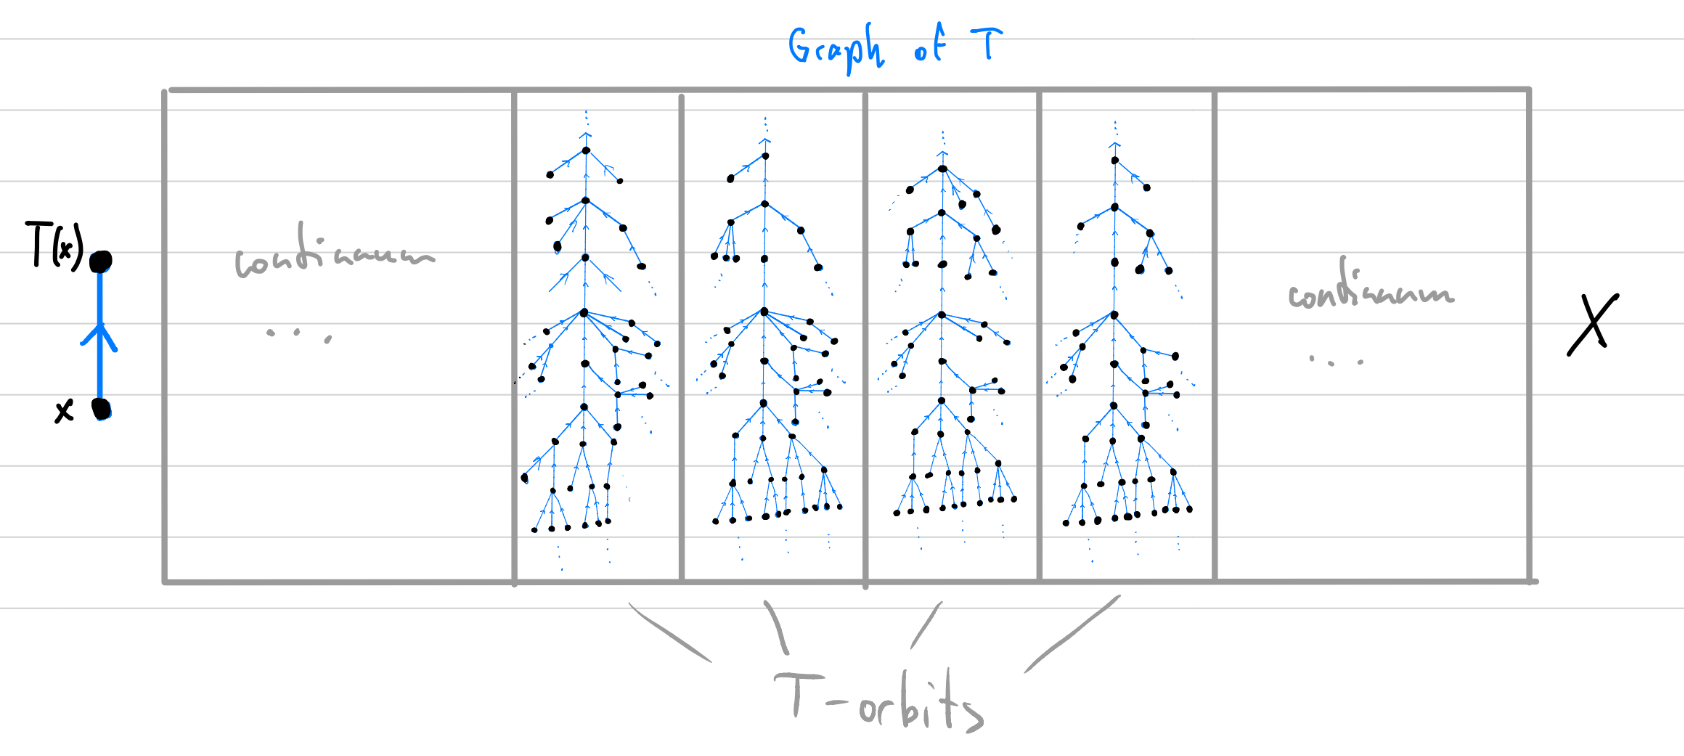
\includegraphics[width=1\linewidth]{T-orbits.PNG}
    \caption{T-orbits}
    \label{T-orbits}
\end{figure}

For example, if we focus on a fixed $x\in X$, then the Birkhoff Ergodic Theorem involves takings the averages on the red-line in Figure \ref{forward-orbit} which represents the forward-orbit of $x$\\

\begin{figure}[h]
    \centering
    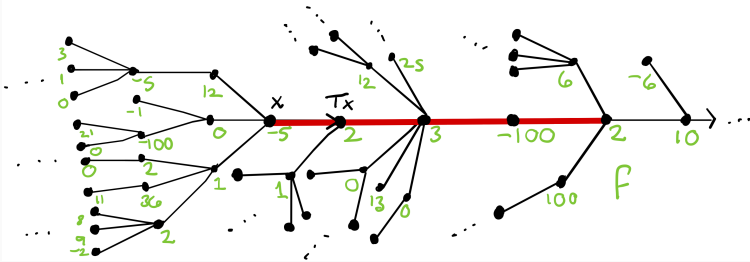
\includegraphics[width=1\linewidth]{forward-orbit.PNG}
    \caption{Forward-orbit of $x$}
    \label{forward-orbit}
\end{figure}

The Backward Triangle Theorem involves however taking the \textit{weighted} average on backward-orbits of $x$.

\begin{definition}[T-Backward-orbit]
    Let $T:X\to X$ be a transformation and $x$ an element of $X$, then the \textit{T-backward-orbit} of $x$ (or simply \textit{backward-orbit} of $x$) is the set 
    $$\rhd_T^n(x) := \bigcup_{n=0}T^{-n}\{x\}$$
\end{definition}

We can now state the Backward Triangle Theorem.

\begin{theorem}[Backward Triangle Theorem]
    A countable-to-one pmp transformation $T:X\to X$ is ergodic iff 
    $$\lim_{n\to\infty}\frac{1}{n+1}\sum_{y\in\rhd_T^n(x)}f(y)w_x(y) =\int_Xfd\mu$$ for all $f\in L^1(X,\mu)$ and a.e $x\in X$.
\end{theorem}

In this theorem, the weight function $w:E_T\to\mathbb{R}$ is called the \textit{Radon-Nikodym cocycle} and satisfies the following properties :
\begin{itemize}
    \item $w_x(y)\cdot w_y(z) = w_x(z)$ for all $xE_TyE_Tz$\\
    \item for any Borel bijection $\gamma : A\to B$ with $A,B\subset X$ and $\gamma \subset E_T$:
    $$\mu(\gamma(A))= \int_Aw_x(\gamma (x))d\mu(x)$$
\end{itemize}
It is a good way of assigning a relative weight between the elements of $X$ that are $E_T$-equivalent.\\

However, the previous theorem can be generalized to any backward trees instead of backward triangles. From this idea, we get the Backward Trees Theorem :

\begin{theorem}[Backward Trees Theorem]
    A countable-to-one pmp transformation $T:X\to X$ is ergodic iff 
    $$\frac{1}{w_x(\tau_x)}\sum_{y\in\tau_x}f(y)w_x(y) \to\int_Xfd\mu \quad \text{ as } w_x(\tau_x)\to\infty$$ for all $f\in L^1(X,\mu)$ and a.e $x\in X$ and where $\tau_x$ ranges over finite subtrees in $\rhd_T^n(x)$.
\end{theorem}

These two theorems (the first one is a special case of the second one) can also be proved using the Local-Bridge + Invariance + Tiling technique used previously to prove the Birkhoff Ergodic Theorem.

\subsection{Group Actions Ergodic Theorems}
In this subsection, consider a probability space $(X,\mu)$. Using group actions, we can generalize the Birkhoff Ergodic Theorem in many ways. First, let's define ergodicity for equivalence relations and group actions.

\begin{definition}[Ergodicity for equivalence relation]
    Let $E$ be an equivalence relation, then we say that $E$ is \textit{ergodic} if each $E$-invariant (which must be union of $E$-equivalence classes) measurable set is null or conull. 
\end{definition}

\begin{definition}[Ergodicity for Group Actions]
    A group acting on $X$ is \textit{ergodic} if its orbits equivalence relation is ergodic.
\end{definition}

Using these new definitions, we can now restate the Birkhoff Ergodic Theorem :

\begin{theorem}[Birkhoff Ergodic Theorem]
    A pmp action $\mathbb{Z}$ on $(X,\mu)$ is ergodic iff 
    $$\lim_{n\to\infty}\sum_{y\in F_n\cdot x}f(y)=\int_Xfd\mu$$
    for all $f\in L^1(X,\mu)$ and a.e $x\in X$ where $F_n = \{0, ...,n\}$.
\end{theorem}

In fact, we can generalize this theorem to any pmp actions of an amenable group along tempered F$\emptyset$lner sequences by the Lindenstrauss Theorem. The free groups are non amenable, unfortunately, it was proved by Terence Tao that the pointwwise ergodic theorem fails for such groups.

\newpage

% ------------------------------------------------------------------------------
% Reference and Cited Works
% ------------------------------------------------------------------------------



\begin{thebibliography}{9}

\bibitem{BN2015}
Bowen and Nevo (2015), Amenable Equivalence Relations and the construction of ergodic averages for group actions.

\bibitem{AT}
Anush Tserunyan (2024), A descriptive approach to pointwise ergodic theorems

\end{thebibliography}

\end{document}
